\chapter{Desarrollo del sistema}
    \label{chapter:desarrollo}

    \chapquote{¿Quién dijo miedo habiendo hospitales?}{Sabiduría popular de la ETSISI}
    
    \section{Project Blastoff}
        \todo{descripcion del blastoff}
        
        \subsection{Inception Deck}
            El \textit{Inception Deck} (también conocido como \textit{Agile Inception}) \cite{rasmusson_agile_2010} \cite{lopez_mendoza_agile_2021} es un conjunto de actividades propio de las metodologías ágiles, las cuales tienen como objetivo establecer inequívocamente los propósitos del proyecto y sus expectativas, a través de la comunicación entre todas las personas involucradas de alguna manera en el proyecto.
            
            Más concretamente, el \textit{Inception Deck} es un conjunto de 10 complejos ejercicios y preguntas, los cuales permiten unificar todas las visiones del producto hacia una sola, asegurando que el equipo avance en sintonía hacia una misma dirección.
        
            Dichas dinámicas son las siguientes:
            \begin{itemize}
                \item ¿Por qué estamos aquí? (\textit{Why are we here?}): describe los motivos principales por los que se realiza este proyecto, y cómo hemos llegado hasta este punto.
                \item \textit{Elevator Pitch}: consiste en transmitir resumida y atractivamente la idea de nuestro proyecto condensada en unos 30 segundos (lo que podría durar un viaje en ascensor, de ahí el nombre) para captar la atención de otras personas. En este pequeño discurso se muestra el problema a resolver, cómo se pretende solventar y cuál es el valor diferencial que tiene nuestra idea y/o equipo, para alentar al oyente a colaborar con el mismo.
                \item Diseñar una caja de producto (\textit{Design a Product Box}): obliga a imaginar nuestro proyecto encapsulado en un cartel publicitario, buscando para ello los mensajes e imágenes para promocionar el producto.
                \item Crear una lista de NOes (\textit{Create a NOT list}): delimita los límites del proyecto estableciendo lo que no se va a realizar en el mismo.
                \item Conoce a tus vecinos (\textit{Meet your neighbors}): esclarece las personas o equipos de los cuales depende el éxito de nuestro proyecto.
                \item Haz ver la solución (\textit{Show the solution}): diseña a alto nivel la arquitectura técnica del producto, de forma legible para todas las partes del proyecto.
                \item ¿Qué nos quita el sueño? (\textit{Ask what keep us up at night}): identifica los posibles riesgos a los que se enfrentará nuestro proyecto que pueden afectar a su desarrollo y éxito. Se diferencia entre los riesgos en los que podemos influir y en los que no, para decidir medidas para mitigar su posible impacto en el caso de los primeros y concienciar acerca de los segundos.
                \item Tómale las medidas (\textit{Size it up}): estimación a grandes rasgos del orden de magnitud temporal del proyecto, para controlar las expectativas del mismo.
                \item Ser claros en qué vamos a dar (\textit{Be clear on what's going to give}): determina las prioridades del proyecto en factores clave como el tiempo, alcance, presupuesto o calidad entre otros, junto a su flexibilidad para redimensionar el proyecto si es necesario.
                \item ¿Cuánto va a costar? (\textit{Show what it's going to take}): desarrollo un presupuesto aproximado tanto en dinero como en personal y recursos si no se realizó previamente. En caso contrario, se discute la viabilidad el mismo y del proyecto.
                
            \end{itemize}
            
            A continuación se describe el resultado de dichas actividades para este proyecto.
            
            \subsubsection{Why are we here?}
                La Salud Mental es un área de la salud cuya visibilización aumenta cada día, pero que aún sigue recubierta de estigma y carece de recursos suficientes. Organizaciones como la Organización Mundial de la Salud y la Confederación de Salud Mental de España han realizado informes e infografías donde se presentan datos sobre este problema tan silencioso, grave y desconocido.
                
                En nuestro país, el 6,7\% de la población está afectada por la ansiedad, exactamente la misma cifra de personas con depresión. Casi la mitad de los españoles de entre 15 y 29 años (48,9\%) considera que ha tenido algún problema de salud mental, mientras que más de la mitad de las personas con trastorno mental que necesitan tratamiento no lo reciben.
                
                A nivel mundial, el 12,5\% de todos los problemas de salud está representado por los trastornos mentales, una cifra mayor a la del cáncer y los problemas cardiovasculares. Más de 300 millones de personas viven en el mundo con depresión, un problema que se ha aumentado en un 18,4\% entre 2005 y 2015; mientras que 800.000 personas se suicidan cada año, siendo la segunda causa de muerte en personas de 15 a 29 años.
                
                Con semejantes estadísticas, queda un largo camino por recorrer para que la sociedad considere a la salud mental como un área de salud igual de importante que las demás. Esto se manifiesta enormemente en la falta de atención a sus síntomas, lo que conlleva faltas crónicas de tratamiento entre la población.
                
                Desde la Informática podemos acceder a numerosos datos, tanto de comportamiento de una persona con su móvil, como datos sobre su estado físico con la generalización de dispositivos conocidos como \textit{wearables} (generalmente una pulsera o reloj inteligente equipado con sensores biométricos). 
                
                Bajo esta premisa se han publicado estudios \cite{schmidt_introducing_2018} \cite{boukhechba_demonicsalmon_2018} \cite{hickey_smart_2021} \cite{rui_studentlife_2014}  que avalan que a partir de dichos datos se estimar por ejemplo si una persona tiene estrés, lo que supone un primer paso para la detección de problemas de salud mental.
                
                Asimismo, los fabricantes de los dispositivos \textit{wearables} ofrecen aplicaciones en las que se pueden consultar los datos recolectados, pero no ofrecen datos acerca de la salud mental, y tampoco son ofrecidos en los smartphones. 
                
                \textbf{Por este motivo estamos aquí}: para realizar una aplicación que aunando software y hardware pueda alertar de síntomas de problemas de salud mental, para que dicha persona sea consciente de que su salud mental puede estar deteriorándose y quizás necesite ayuda profesional.
                
            \subsubsection{Elevator pitch}
                Se estima que el 25\% de las personas tendrá un trastorno mental a lo largo de su vida, y entre ellas, entre el 35\% y el 50\% no reciben tratamiento o no es el adecuado. Para la comunidad universitaria presentamos el Sistema para el Bienestar Emocional, una aplicación que permite obtener tu nivel de estrés teniendo en cuenta el uso del móvil y opcionalmente la información de \textit{\textit{wearables}}. 
                
                A diferencia de otras aplicaciones, no nos fijamos únicamente en el dato de un sensor invasivo ni comunicamos datos con terceras empresas, nuestro producto es una aplicación \textit{open source}, por lo que puedes modificarla a tu antojo, que proporciona resultados más elaborados y precisos y elabora recomendaciones para tu situación mental.
                
            \subsubsection{Product Box}
                TODO
                \todo{nos falta la imagen cuando esté disponible}
                
            \subsubsection{NOT list}
                \vspace*{5mm}
                \begin{tabularx}{\textwidth}{ | X | X | }
                    \hline
                    Dentro del alcance & Fuera del alcance \\
                    \hline
                        \textbullet\ Desarrollo de la aplicación de usuario para dispositivos Android en el lenguaje de programación Kotlin. 
                        & 
                        \textbullet\ Desarrollo de la aplicación para terminales con otro sistema operativo, como iOS. \\
                        
                        \textbullet\ Lectura de datos biométricos del usuario: ritmo cardíaco y sus variaciones, sueño, actividad física. 
                        & 
                        \textbullet\ Retro-aprendizaje del modelo de Inteligencia Artificial para un usuario en particular. \\
                        
                        \textbullet\ Obtención de datos del móvil: sueño, uso de aplicaciones. 
                        & 
                        \textbullet\ Evolución del modelo de Inteligencia Artificial tras la prueba piloto. \\
                        
                        \textbullet\ Comunicación de resultados a los usuarios mediante notificaciones. 
                        & 
                        \textbullet\ Utilización de mecanismos de \textit{edge computing} en la aplicación de usuario. \\
                        
                        \textbullet\ Visualización tanto del estado de bienestar emocional actual como de su evolución. 
                        & 
                        \textbullet\ Implementación de cuentas de usuario para mantener los datos entre dispositivos.\\
                        
                        \textbullet\ \textit{Layout responsive} de la aplicación para adaptarla a todo tipo de dispositivos. 
                        & 
                        \textbullet\ Realización de ingeniería inversa a las pulseras Xiaomi desde cero. \\
                        
                        \textbullet\ Desarrollo del modo oscuro de la interfaz de la aplicación. 
                        & 
                        \textbullet\ Inclusión de otras pulseras que no dispongan del sistema operativo Wear OS. \\
                        
                        \textbullet\ Conexión de la aplicación con el modelo de Inteligencia Artificial. 
                        & 
                        \textbullet\ Uso de la herramienta Google Fit para obtener datos de dispositivos. \\
                        
                        \textbullet\ Aporte de los datos de los usuarios para entrenar el modelo de Inteligencia Artificial. 
                        & 
                        \textbullet\ Lectura de sensores de estrés y oxígeno en sangre por ser invasivos de cara al usuario. \\
                        
                        \textbullet\ Validación mediante tests con cuestionarios para corroborar los resultados obtenidos.
                        & 
                        \textbullet\ Utilización de escáneres cerebrales u otros dispositivos similares. \\
                        
                        \textbullet\ Realización profesional de la gestión de proyecto siguiendo metodologías ágiles. 
                        &  \\
                        
                        %\textbullet\ Modelo en local de Inteligencia Artificial
                        %&  \\
                    \hline
                    \multicolumn{2}{| c |}{No resuelto}\\
                    \hline
                    \multicolumn{2}{| c |}{ }\\
                    \hline
                    \caption{Lista de NOes del proyecto}
                    \label{tab:dev:noes}
                    
                \end{tabularx}
                
            \subsubsection{Meet your neighbors}
                \vspace{-\topsep+5mm}
                \begin{itemize}
                    \item Estudiantes de la universidad como usuarios del sistema.
                    \item Profesores de la universidad como usuarios y/o promotores del sistema.
                    \item Responsables de la infraestructura de la universidad para poder entrenar el modelo de Inteligencia Artificial.
                    \item Fabricantes tanto de los \textit{wearables} como de los smartphones.
                    \item Desarrolladores del S.O. Android y sus API oficiales.
                    \item Futuros desarrolladores del proyecto, como estudiantes de la escuela para sus proyectos Fin de Titulación; bien a nivel de aplicación o de Inteligencia Artificial.
                    \item Subdirección de Asuntos Económicos de la ETSISI como responsables de la compra de material hardware para este proyecto.
                    \item Consultores internos sobre desarrollo de aplicaciones móviles, ingeniería de software e integración de componentes hardware para transmitir los conocimientos necesarios para continuar el proyecto/resultados del mismo.
                \end{itemize}
                
            \subsubsection{Show the solution}
                
                \vspace*{5mm}
                \begin{figure}[H]
                    \centering
                    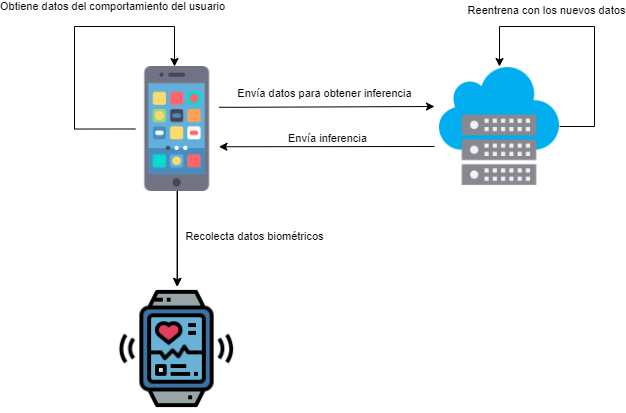
\includegraphics[width=0.66\textwidth]{figures/inception-deck/Componentes.png}
                    \caption{Componentes básicos del sistema}
                    \label{fig:dev:componentes}
                \end{figure}
                
                \vspace*{5mm}
                \begin{figure}[H]
                    \centering
                    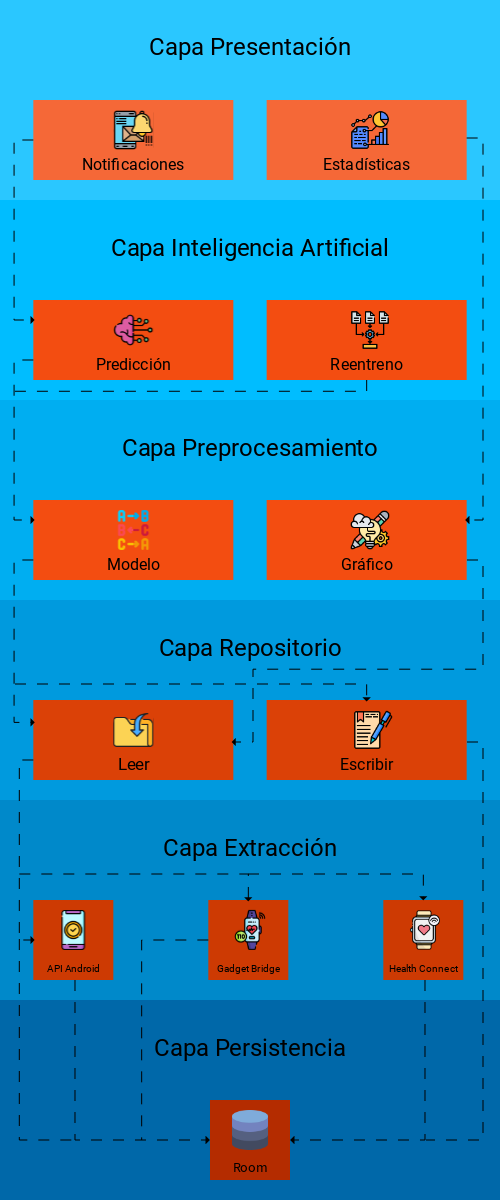
\includegraphics[width=0.475\textwidth]{figures/inception-deck/Pila.png}
                    \caption{Pila con la arquitectura del sistema}
                    \label{fig:dev:arquitecturaPila}
                \end{figure}
            
            \subsubsection{Up at night}
                
                \vspace*{5mm}
                \begin{tabularx}{\textwidth}{ | X | X | }
                    \hline
                    Riesgos en los que podemos influir & Riesgos en los que no podemos influir \\
                    \hline
                        \textbullet\ Realización de pruebas exhaustivas tanto del \textit{backend} como de la interfaz gráfica de usuario.
                        & 
                        \textbullet\ Problemas de compatibilidad entre las versiones de Android.	 \\
                        
                        \textbullet\ Participación de voluntarios que aporten datos al estudio con los que mejorar la precisión y evitar sesgos.
                        &
                        \textbullet\ Muestra de estudiantes variada y contrastada participando en el proyecto. \\
                        
                        \textbullet\ Elaboración de unos términos y condiciones legales acerca de los datos obtenidos en el proyecto.
                        & 
                        \textbullet\ Soportes de los fabricantes de \textit{wearables} (en especial Samsung) a Health Connect. \\
                        
                        \textbullet\ Accesibilidad correcta de la aplicación. 
                        & 
                        \textbullet\ Funcionamiento de las pulseras Xiaomi en aplicaciones no oficiales. \\
                        
                        \textbullet\ Elaboración de un diseño coherente a nivel UX/UI de la aplicación. 
                        & 
                        \textbullet\ Disponibilidad de los datos del móvil y de los \textit{wearables}. \\
                        
                        \textbullet\ Comunicación y difusión eficaz del proyecto en la escuela, en la defensa de este TFM y en redes sociales. 
                        & 
                        \textbullet\ Fiabilidad suficiente de los datos obtenidos por el móvil y los \textit{wearables}. \\
                        
                        \textbullet\ Continuidad del proyecto después del presente TFM para, entre otros, publicar una aplicación en iOS.
                        &
                        \textbullet\ Incumplimiento de la planificación por circunstancias ajenas al proyecto. \\
                        
                        \textbullet\ Definición clara de la arquitectura y de los procesos de mantenimiento y ampliación de la aplicación.
                        &
                        \textbullet\ Retrasos en la entrega del hardware necesario para el sistema. \\
                        
                        
                        \textbullet\ Mantenimiento futuro de la aplicación con las nuevas versiones de Android. 
                        & 
                        \textbullet\ Ausencia de fallos al publicar la aplicación en la Google Play Store. \\
                    
                        
                        \textbullet\ Potencia de cómputo suficiente para entrenar el modelo de Inteligencia Artificial
                        & 
                        \textbullet\ Precisión insuficiente del modelo de Inteligencia Artificial para ser utilizado en un entorno real.\\


                    \hline
                    
                    \caption{Riesgos del proyecto}
                    \label{tab:dev:riesgos}
                \end{tabularx}
                
            \subsubsection{Size it up}
                %begin{landscape}
                \vspace*{5mm}
                \begin{figure}[H]
                    \centering
                    %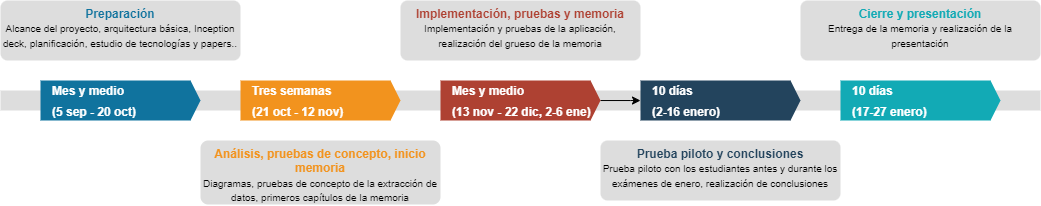
\includegraphics[width=\textheight,angle=90,origin=c]{figures/inception-deck/Size up.png}
                    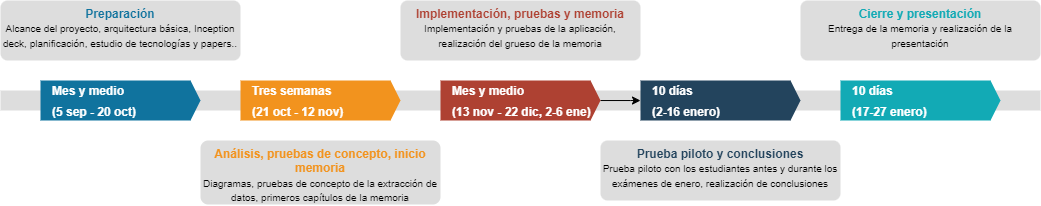
\includegraphics[width=\textwidth]{figures/inception-deck/Size up.png}
                    \caption{Dimensionamiento aproximado del proyecto}
                    \label{fig:dev:sizeItUp}
                \end{figure}
                %\end{landscape}
            \subsubsection{What's going to give}
                
                \vspace*{5mm}
                \begin{tabularx}{\textwidth}{ | >{\hsize=.34\hsize}X | >{\hsize=.14\hsize}X | >{\hsize=.52\hsize} X | }
                    \hline
                        Aspecto 
                        & 
                        Importancia  
                        & 
                        Implicaciones \\
                    \hline
                        Detalle de la documentación
                        & 
                        Media  
                        & 
                        Se desea que la memoria explique detalladamente las cuestiones importantes del proyecto y cubra todo lo realizado en el mismo, pero no es necesario en detalles menores ni se pretende que la memoria sea excesivamente larga. \\
                    \hline
                        Alcance de la implementación 
                        & 
                        Baja - media  
                        & 
                        Una vez realizada la conexión con las API de Android y con el hardware concedido, se puede establecer flexibilidad con el alcance del prototipo. \\
                    \hline
                        Calidad 
                        & 
                        Media - alta  
                        & 
                        Se deben realizar pruebas detalladas y obtener métricas de calidad del software implementado, pero se permite cierta flexibilidad en las mismas sobre el software que maneje el hardware del proyecto por su alta dificultad. \\
                    \hline
                        Comunicación del proyecto 
                        & 
                        Alta  
                        & 
                        Se necesitan usuarios para la prueba piloto y para obtener retroalimentación del proyecto. No obstante, si bien se desea que el proyecto sea continuado, no es estrictamente necesario.\\
                    \hline
                        Experiencia de usuario 
                        & 
                        Media  
                        & 
                        La aplicación debe ser intuitiva y accesible para el usuario, pero no se necesita que el prototipo tenga un diseño visual (elementos, animaciones, gráficas) muy elaborado y detallado al ser un prototipo. \\
                    \hline
                        Fiabilidad 
                        & 
                        Media  
                        & 
                        No están previstas pruebas exhaustivas con todos los dispositivos compatibles (versiones del SO, dispositivos hardware), por lo que \textit{bugs} leves son admisibles. \\
                    \hline
                        Presupuesto (hardware) 
                        & 
                        Muy alta  
                        & 
                        El presupuesto está cerrado al aprobado, por lo que no se pueden incorporar nuevos componentes. \\
                    \hline
                        Rendimiento 
                        & 
                        Baja - media  
                        & 
                        La optimización del software queda fuera del proyecto, si bien se debe de garantizar un rendimiento mínimo para no afectar la experiencia de usuario. \\
                    \hline
                        Seguridad 
                        & 
                        Alta  
                        & 
                        Si bien los datos del móvil no son personales, los de los \textit{wearables} sí lo son, por lo que deben ser debidamente protegidos tanto en su almacenamiento como en su trasmisión con técnicas estándar. \\
                    \hline
                        Tiempo 
                        & 
                        Muy alta  
                        & 
                        El máster proporciona dos convocatorias fijas en el calendario, y por la situación personal del autor solo puede acudir a la de enero, por lo que el proyecto debe finalizar para esa fecha. \\
                    \hline
                    
                    \caption{Cuestiones y prioridades del proyecto}
                    \label{tab:dev:prioridades}
                \end{tabularx}
            
            
            \subsubsection{What it's going to take}
            
                En el apartado de Tómale las medidas se establecieron las etapas del proyecto, por lo que ya conocemos el tiempo estimado de desarrollo del proyecto: cuatro meses y medio. Asimismo, al ser un Trabajo Final de Máster realizado por una persona se necesita a un único ingeniero para el proyecto.
                
                Durante ese plazo las labores del desarrollador incluyen (pero no se limitan a):
                \begin{itemize}
                    \item Análisis y planteamiento del problema a resolver.
                    \item Diseño de un sistema que combine hardware y software.
                    \item Implementación de una aplicación Android con el lenguaje de programación Kotlin.
                    \item Diseño de interfaces de usuario y experiencia de usuario. 
                    \item Comunicación de smartphones Android con dispositivos \textit{wearables} mediante Bluetooth.
                    \item Realización de pruebas unitarias, funcionales y de integración.
                    \item Uso de sistemas de control de versiones, como Github.
                    \item Desarrollo de un pipeline CI/CD.
                    \item Aplicación de metodologías ágiles.
                \end{itemize}
                
                No obstante, son labores que puede desarrollar un perfil con formación universitaria en Informática, ya que al ser un proyecto relativamente breve no se necesita de personal especializado en análisis, pruebas, etc. 
                
                Por tanto, se supone que dicho perfil es un Android Developer y que su salario es el promedio. Según la conocida web de empleo Glassdoor, dicho salario medio en Madrid es de 33.000 €/año, por lo que su salario prorrateado es de 12.375€. Asimismo, hay que sumar el presupuesto concedido por la universidad, que asciende a 460€.
                
                Por tanto, la estimación del coste total del proyecto es de 12.835€.

        
            